%%%%%%%%%%%%%%%%%%%% author.tex %%%%%%%%%%%%%%%%%%%%%%%%%%%%%%%%%%%
%
% sample root file for your "contribution" to a proceedings volume
%
% Use this file as a template for your own input.
%
%%%%%%%%%%%%%%%% Springer %%%%%%%%%%%%%%%%%%%%%%%%%%%%%%%%%%


\documentclass{svproc}
%
% RECOMMENDED %%%%%%%%%%%%%%%%%%%%%%%%%%%%%%%%%%%%%%%%%%%%%%%%%%%
%

% to typeset URLs, URIs, and DOIs
\usepackage{url}
\usepackage{graphicx,url}
\usepackage[utf8]{inputenc}
\usepackage{subfig}
\def\UrlFont{\rmfamily}

\begin{document}
\mainmatter              % start of a contribution
%
%\title{Análise de Desempenho do MongoDB Utilizando Diferentes \emph{drivers} em um Ambiente de Aplicação Node.js}
%\title{Análise de Desempenho dos drivers do MongoDB em um Ambiente de Aplicação Node.js}
%\title{Análise de Desempenho de Aplicação Node.js utilizando drivers do MongoDB}
\title{Analysis of Node.js Application Performance using MongoDB drivers}
%
%\titlerunning{Análise de Desempenho dos drivers do MongoDB em um Ambiente de Aplicação Node.js}  % abbreviated title (for running head)
%\titlerunning{Análise de Desempenho de Aplicação Node.js}
\titlerunning{Analysis of Node.js Application Performance}
%                                     also used for the TOC unless
%                                     \toctitle is used
%
\author{Leandro Ungari Cayres\inst{1} \and Bruno Santos de Lima\inst{1} Rogério Eduardo Garcia\inst{1} \and Ronaldo Celso Messias Correia\inst{1}}
%\author{OMITTED}
%
\authorrunning{Cayres et al.} % abbreviated author list (for running head)
%\authorrunning{OMITTED} % abbreviated author list (for running head)
%
%%%% list of authors for the TOC (use if author list has to be modified)
\tocauthor{Leandro Ungari Cayres, Bruno Santos de Lima, Rogério Eduardo Garcia, and Ronaldo Celso Messias Correia}
%\tocauthor{OMITTED}
%
\institute{Faculty of Science and Technology -- São Paulo State University (UNESP), Presidente Prudente -- SP, Brazil,\\
%\institute{OMITTED\\
\email{\{leandro.ungari,bruno.s.lima,rogerio.garcia,ronaldo.correia\}@unesp.br}
%\email{OMITTED}
}

\maketitle % typeset the title of the contribution

\begin{abstract}
At the last few years, the usage of NoSQL databases has increased, and consequently, the need for integrating with different programming languages. In that way, database drivers provide an API to perform database operations, which may impact on the performance of applications. In this article, we present a comparative study between two main drivers solutions to MongoDB in Node.js, through the evaluation of CRUD tests based on quantitative metrics (time execution, memory consumption, and CPU usage). Our results show which, under quantitative analysis, the MongoClient driver has presented a better performance than Mongoose driver in the considered scenarios, which may imply as the best alternative in the development of Node.js applications.
\keywords{Performance, Node.js application, MongoDB, drivers, NoSQL databases}
\end{abstract}
%

\section{Introduction}
\label{sec:introducao}

%Nos últimos anos, o crescimento no volume de dados mudou a utilização desses por empresas e organizações. Inicialmente como agentes passivos, relacionados às regras de negócio empresarial; os dados se tornaram potenciais oportunidades de lucro e obtenção de conhecimento através de processos de análise de dados.
At the last few years, the growth of data volume has changed the perspective of how organizations behavior, from simple data recording to potential advantage in competitive markets.

%O advento do~\emph{Big Data} não implicou somente em maior espaço de armazenamento, mas em uma mudança de organização, considerando características como volume, variedade, velocidade e valores~\cite{ward2013undefined}. 
%A arquitetura dos tradicionais Bancos de Dados Relacionais são baseadas em propriedades ACID (\textit{Atomicity},~\textit{Consistency},~\textit{Isolation} e~\textit{Durability}), contudo, em ambientes de~\emph{Big Data} a alta consistência provida afeta diretamente os aspectos de disponibilidade e eficiência, que são primordiais, devido ao alto volume, variedade e velocidade~\cite{aparicio:2016}. 
%Nesse cenário, os Banco de Dados \textit{NoSQL} (\emph{Not only SQL}) proporcionam maior flexibilidade estrutural, escalabilidade, suporte a replicação e consistência eventual, desse modo, surgem como alternativas de destaque~\cite{han2011survey}. 
This event, known as Big Data, not only implies in large storage but also perspectives related to variety, velocity, and value~\cite{ward2013undefined}. The traditional architecture of relational databases based on ACID (atomicity, consistency, isolation, and durability) properties, which affect the aspects related to availability and efficiency directly in Big Data environments~\cite{aparicio:2016}. 
The non-relational databases (NoSQL) have been proposed oo solve the side-effects, and allowing more structural flexibility, scalability, and support to replication and eventual consistency~\cite{han2011survey}.
  
%Neste contexto, para os diferentes ambientes de desenvolvimento e linguagens de programação,~\emph{drivers} tem sido desenvolvidos de modo a viabilizar e apoiar execução de operações pertences aos bancos de dados. Entretanto, em muitos casos, além de recentes, os~\emph{drivers} apresentam limitações em sua implementações, falhas de entendimento e efeitos colaterais no acesso aos dados~\cite{rafique:2018}. 
%Assim, a decisão de qual combinação entre Banco de Dados \textit{NoSQL} e~\emph{driver} a ser empregada pode ser um problema, devido ao desconhecimento dos pontos positivos e negativos.
In this context of development environments and programming languages, a variety of database drivers aim to support the execution of the internal database operations.
However, in many cases, the development of these drivers are very recent and may present defects or limitations, which results in side-effects to the access and manipulation of data~\cite{rafique:2018}.
Thus, the usage decision of which NoSQL database and driver may impact on the performance, due to unknown factors previously.


%Neste artigo, por meio de um experimento comparativo de desempenho, é realizado a avaliação das duas principais soluções de~\emph{drivers} para o MongoDB~\footnote{https://www.mongodb.com/}, respectivamente \emph{MongoClient}~\footnote{https://mongodb.github.io/node-mongodb-native/} e \emph{Mongoose}~\footnote{https://mongoosejs.com/}, em ambientes de aplicação Node.js. 
%O principal fator considerado para a realização dessa análise consiste na definição prévia de esquema para a manipulação dos dados em operações de CRUD (\emph{create}-\emph{read}-\emph{update}-\emph{delete}). Conceitualmente, os Bancos de Dados~\textit{NoSQL} não requerem essa predefinição, proporcionando flexibilidade, entretanto, não existe nada que impeça sua utilização, principalmente quanto a respeito do desempenho; possibilitando algum impacto relevante.
In this work, we conduct a comparative study of performance between MongoClient~\footnote{https://mongodb.github.io/node-mongodb-native/} and Mongoose~\footnote{https://mongoosejs.com/}, both solutions of database drivers to MongoDB~\footnote{https://www.mongodb.com/} in Node.js applications.
The main difference between them is the predefinition of schema, a factor which is not mandatory in the majority of NoSQL databases, and MongoDB too; but in one of these drivers is required.
In that way, this experimental study analyses the impact of each driver at CRUD (create, read, update, and delete) operations. 

%A escolha do MongoDB ocorreu devido a sua crescente investigação por parte da comunidade cientifica em diversas pesquisas~\cite{patil:2017,jung:2015,ongo:2018,kanade2014study}; além de ser uma das principais opções de armazenamento orientada a documentos. Quanto ao Node.js, mesmo recente, alguns trabalhos apontam a sua viabilidade tecnológica no desenvolvimento de aplicações~\cite{chaniotis2015node}. Com essa escolha, tanto aplicação quanto Banco de Dados utilizam \textit{JavaScript}, uniformizando o sistema em termos de linguagem de programação.

The choose of MongoDB based on a crescent number of studies in the research community, and also it is the main option of the document-oriented database.
In about Node.js, despite recent development, it presents technical viability to implement robust applications.
Also, the database system and application lead to uniformization, because both are implemented in JavaScript.

%Este trabalho busca analisar o impacto causado no desempenho de uma aplicação Node.js que faz uso do Banco de Dados~\emph{NoSQL} MongoDB, ao utilizar os dois diferentes drivers disponíveis para o Banco de Dados em questão. 
%Este trabalho está situado como único presente na literatura com investigação na perspectiva de avaliar a influência de diferentes drivers do MongoDB no desempenho de uma aplicação Node.js, uma vez que, os demais trabalhos investigam outros aspectos relacionados ao MongoDB como por exemplo: comparação de desempenho com outros Bancos de Dados~\cite{jung:2015,patil:2017,ongo:2018} e influência na performance do Banco de Dados ao utilizar diferentes modelagens de dados~\cite{kanade2014study}.
This study is unique in the investigation of effects of performance in different database drivers in Node.js application since the other works have analyzed performance between database~\cite{jung:2015,patil:2017,ongo:2018} or the modeling impact on the performance in databases~\cite{kanade2014study}.

%Este artigo está organizado do seguinte modo: na Seção~\ref{section:fundamentacao} são apresentados conceitos de Banco de Dados~\emph{NoSQL}, MongoDB e seus \emph{drivers}.
%A Seção~\ref{section:experimento} é apresentada a estruturação do experimento. 
%Na Seção~\ref{section:resultados} são descritos os resultados quantitativos obtidos, cuja a análise está situada na Seção~\ref{section:discussao}. Por fim, a Seção~\ref{section:consideracoes} expressa as considerações finais.
The remaining of this article as follows: Section~\ref{section:fundamentacao} presents relevant topics related to NoSQL databases and MongoDB. Section~\ref{section:experimento} presents the conception of an experimental project. Section~\ref{section:resultados} describes the obtained results, which analysis is in Section~\ref{section:discussao}. Finally, Section~\ref{section:consideracoes} presents the final remarks of the presented study.

\section{Background}
\label{section:fundamentacao}

%Nesta seção, são discutidos alguns conceitos fundamentais para o trabalho: Bancos de Dados~\emph{NoSQL}, as características do MongoDB e dos \emph{drivers} \emph{MongoClient} e \emph{Mongoose}. 

\subsection{NoSQL Databases}
\label{subsection:nao-relacional}

%Os Bancos de Dados~\emph{NoSQL} foram desenvolvidos visando armazenar e processar grandes volumes de dados. 
%Em linhas gerais os bancos de dados~\emph{NoSQL} são livres de esquematizações e mais propícios a lidar com dados não estruturados como e-mails, documentos e mídias sociais de maneira eficiente~\cite{mohamed:2014,ramesh:2016}.

NoSQL databases were developed to fulfill storage requirements in big data environments. In that way, their schemaless data structure provides more flexibility to many applications, such as e-mails, documents, and social media content~\cite{mohamed:2014,ramesh:2016}.

%O termo~\emph{NoSQL} é utilizado para se referir a uma ampla variedade de armazenamentos de dados, em que as restrições de transação ACID foram suavizadas permitindo melhor dimensionamento e desempenho horizontal~\cite{rafique:2018}, proporcionando esquemas menos estruturados, suporte a operações de junção, alta escalabilidade, modelagem de dados simples com linguagem de consulta simples~\cite{ramesh:2016}. 
%Os bancos de dados~\emph{NoSQL} são categorizados em: armazenamento de documentos, famílias de colunas, chave/valor, grafos e multimodais~\cite{aparicio:2016}.
The NoSQL term refers to wide variety of storage systems, which are non-strict ruled by ACID properties, to allow better data structure and horizontal performance~\cite{rafique:2018}, join operations, high scalability, and data modeling by simplified queries~\cite{ramesh:2016}.
The relational databases are divided into four categories: document-oriented, column-oriented, key/value-oriented, graph-oriented, and multimodal.

%Este trabalho tem como foco a categoria orientada a documentos, a qual possui modelagem de dados estreitamente relacionados a programação orientada a objetos, possibilitando flexibilidade no armazenamento de registros com atributos distintos, sendo útil na modelagem de dados não-estruturados e polimórficos. Permite consultas robustas, em que qualquer combinação de campos no documento pode ser realizada~\cite{patil:2017}. Os dados são organizados em coleções de documentos, as quais utilizam uma estrutura semelhante a JSON (\emph{JavaScript Object Notation}) ou XML (\emph{Extensible Markup Language}).

This work focus on oriented-documents databases, which modeling is similar to object-oriented data definition using registers with fields and complex operations~\cite{patil:2017}. 
Each database contains collections, each collection defines similar content groups, and each item corresponds to a document structured as JSON (JavaScript Object Notation) or XML (Extensible Markup Language).

\subsection{MongoDB}

%O MongoDB é um Banco de Dados orientado a documentos que possui código-aberto, o qual provê funcionalidades como ordenação, indexação secundária e consultas de intervalo~\cite{membrey2011definitive}.

%O banco de dados não impõe um esquema prévio, entretanto, normalmente todos os documentos em uma coleção são de propósito semelhante ou relacionado~\cite{kanade2014study,lutu2015big}. Há duas abordagens para modelagem de documentos:

MongoDB is an open-source document-oriented database, which provides besides storage functionalities such as data sorting, secondary indexing, and interval queries~\cite{membrey2011definitive}.
It does not require a defined schema, despite the similarity of elements into a collection~\cite{kanade2014study,lutu2015big}. There are two main approaches to document modeling:

%\begin{itemize}
%\item \textbf{Modelo de dados incorporado:} Os dados relacionados são incorporados em uma única estrutura ou documento. Esses esquemas são geralmente conhecidos como modelos sem normalização. %REFERENCIAR
%\item \textbf{Modelo de dados normalizado:} Os dados possuem referências de documentos para registrar relacionamentos entre esses, mas a combinação de documentos deve ser feita diretamente no código-fonte da aplicação. %REFERENCIAR
%\end{itemize}

\begin{itemize}
\item~\textbf{Embedded data modeling:} the data are defined in a unique data structure or document, which results in a high concentration of data.
\item~\textbf{Normalized data modeling:} the data have references among documents to represents relationships.     
\end{itemize}

%O armazenamento dos dados ocorre através da serialização de objetos \textit{Javascript}, também conhecidos como JSON, cuja implementação interna utiliza uma codificação binária chamada BSON\footnote{http://bsonspec.org/}. O banco de dados MongoDB disponibiliza diversos~\emph{drivers} para linguagens de programação como Java, C++, C\#, PHP e Python~\cite{lutu2015big}, e também em Node.js.

The adopted format is JSON, which passes through a codification to binary format BSON~\footnote{http://bsonspec.org/}
. About the integration to programming languages, several drivers are available to Java, C++, C\#, PHP and Python~\cite{lutu2015big}, and Node.js too.

%Dentre os~\emph{drivers} existentes para o MongoDB, tem-se como destaque o \textbf{\textit{MongoClient}}\footnote{https://mongodb.github.io/node-mongodb-native/index.html}, consiste na solução oficial e nativa provida organização, provendo um conjunto de funcionalidades que permite a manipulação dos dados e uso de recursos avançados do sistema. Essa solução é caracterizada pela modelagem documentos-objeto (\emph{ODM -- Object-Document Modeler}) de modo implícito ao banco de dados.

Concerning to Node.js drivers to MongoDB, the first is the MongoClient~\footnote{https://mongodb.github.io/node-mongodb-native/index.html}, the official distributed solution, which provides an API to manipulation of data. The main feature is the implicit document-object modeling, which discards any need for data description.

%Assim como o anterior, o \textbf{\textit{Mongoose}} consiste também em um \emph{driver} para MongoDB, em que provê a modelagem de dados utilizando um mecanismo objeto-relacional (\emph{ORM -- Object Relational Mapping}) utilizado em banco de dados relacionais~\cite{mardan2014boosting}, executando diversas tarefas de verificação e validação dos dados, como nulidade ou tipagem, previamente definidos por meio da elaboração de um esquema.

The second option is the Mongoose~\footnote{https://mongoosejs.com/}, a database driver that provides data modeling based on the object-relational model. It implies that all data elements must describe the definition of attributes, which allows verification of types and validation, nullity checking by a defined schema.

%\subsection{Node.js}
%\label{subsection:nodejs}

%Node.js é uma plataforma construída sob o ambiente de execução para \textit{JavaScript} do navegador Google Chrome, para criação facilitada de aplicações de internet rápidas e escaláveis, baseado em um mecanismo orientado a eventos de entrada e saída não-bloqueante, que viabiliza a interação do usuário enquanto demais tarefas executam em segundo-plano, resultando em aplicações leves e eficientes.
%Cada aplicação Node.js atua como processo comum em um computador, diferentemente da restrição de aplicações \textit{JavaScript} voltadas para navegadores. 

%A Figura~\ref{figure:memoria} apresenta a organização da memória em processos Node.js.

%\begin{figure}[!h]
%    \centering
%    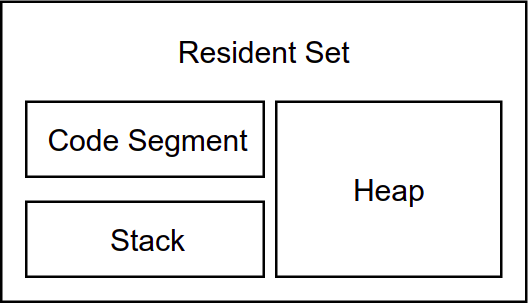
\includegraphics[width=0.35\textwidth]{images/set}
%    \caption{Organização de memória de um processo Node.js -- Adaptado de~\cite{nodememory}.}
%    \label{figure:memoria}
%\end{figure} 

%A região principal é chamada~\emph{Resident Set}, a qual corresponde a toda memória utilizada no processo. Em seguida, tem-se a região~\emph{Code Segment}, a qual armazena todas as instruções definidas para o programa. A próxima região~\emph{Stack} armazena todas as variáveis e estruturas de dados utilizadas durante o tempo de vida dessas. 
%Por fim, tem-se a região~\emph{Heap}, a qual armazena dados específicos como objetos,~\emph{strings} e~\emph{closures}; em geral, cada processo aloca esse região com um tamanho predefinido, contudo essa pode ser utilizada apenas parcialmente ou em sua totalidade~\cite{nodememory}. 

\section{Experimental Setup}
\label{section:experimento}

%Nesta seção é apresentado a composição do experimento comparando os~\emph{drivers} \emph{MongoClient} e \emph{Mongoose} em integração com o MongoDB. 
In this section, we present the definitions of the experimental project which intents to compare the performance of each driver with MongoDB.
Figure~\ref{figure:diagrama-banco} presents the structure of experiment.
%Na Figura~\ref{figure:diagrama-banco} é ilustrado a esquematização do experimento. 

\begin{figure}[!ht]
    \centering
    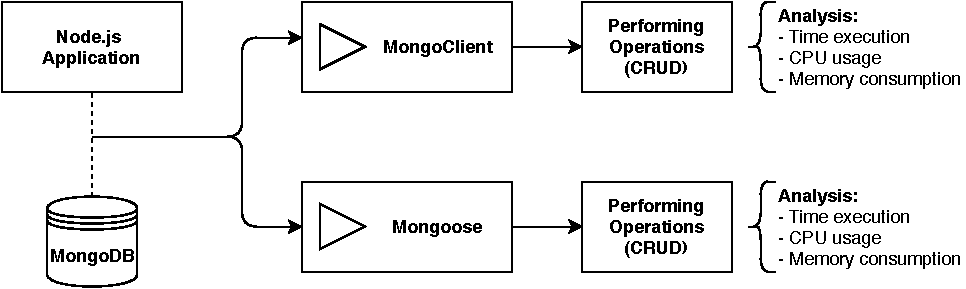
\includegraphics[width=\textwidth]{images/esquema-experimento.pdf}
    \caption{Comparison between MongoDB drivers.}
    \label{figure:diagrama-banco}
\end{figure}
 
%As análises conduzidas visaram identificar qual dupla (MongoDB e \emph{Drive}) possui melhor desempenho em uma aplicação Node.js, ou seja, causa menor impacto no desempenho da aplicação. 
%Além disso, foi investigado se o tamanho médio de cada registro presente no conjunto de dados pode influenciar nesse desempenho e qual a proporção desse impacto.

%Para isso, uma aplicação Node.js foi implementada para a condução dos testes. Essa aplicação é responsável por realizar a conexão com o Banco de Dados MongoDB e executar operações CRUD. A ferramenta de testes implementada em Node.js está disponível para a comunidade científica em: [OMITIDO], podendo ser utilizada em outras pesquisas.%~\footnote{https://github.com/leandroungari/database-driver}.

%As métricas escolhidas para as análises de cada um dos testes conduzidos foram:

The analysis aimed to identify which couple (driver-database) presents better performance in a Node.js application based on quantitative parameters.

We developed a tool to run the test with each driver. In that way, to perform the comparison, the execution flow of application receives a set of parameters, such as driver and number of elements, in follow the database connection is performed and the respective operations. During the tests, we extracted some metrics related to CPU (Central Processing Unit) and memory usage. 
The tool is available in the following open-source repository: \url{https://github.com/leandroungari/database-driver}.

We also defined the performance metrics to evaluate the conducted tests:

%\begin{itemize}
%\item \textbf{Tempo médio de Execução:} Consiste tempo médio total de execução de cada operação específica.
%\item \textbf{Consumo médio de CPU:} Consiste no tempo médio de uso do processador durante a execução de cada operação específica.
%\item \textbf{Consumo médio de Memória:} Consiste na variação média de uso de memória RAM durante a execução de cada operação específica, sendo expressa em kilobytes (KB).
%\end{itemize}

%Por fim, foram formuladas as seguintes de questões de pesquisa que guiaram formalmente as análises executadas: 

%\textbf{QP1} --~\emph{A escolha do driver impacta no desempenho da aplicação Node.js que utiliza o MongoDB, considerando o tempo de execução de cada uma das operações CRUD?}

%\textbf{QP2} --~\emph{A escolha do driver pode influenciar no desempenho da aplicação Node.js que utiliza o MongoDB, considerando o tempo de consumo da CPU ao executar operações CRUD?}

%\textbf{QP3} --~\emph{A escolha do driver impacta de modo relevante no desempenho da aplicação Node.js que utiliza o MongoDB, considerando o consumo médio de memória RAM ao executar operações CRUD?}

\begin{itemize}
\item~\textbf{Average Execution Time:} it defines the average time (in milliseconds) in each operation.
\item~\textbf{Average CPU Usage:} it defines the average time (in milliseconds) usage of CPU during each operation.
\item~\textbf{Average Memory Usage:} it defines the average variation of RAM memory usage (in kilobytes) in each operation.
\end{itemize}

Finally, we formulate a set of research questions to lead the analysis of the results:

\begin{itemize}
\item~\textbf{RQ1} --~\emph{Does the driver selection impact on application performance under time execution?}
\item~\textbf{RQ2} --~\emph{Does the driver selection affect application performance under CPU usage?}
\item~\textbf{RQ3} --~\emph{Does the driver selection impact application performance under RAM memory consumption?}
\end{itemize}

\subsection{Dataset}

%A condução do experimento utilizou um conjunto de dados com cerca 18 mil instâncias.%\footnote{https://www.kaggle.com/karangadiya/fifa19}. 
%Originalmente, todos os registros presentes são compostos por 89 atributos, predominantemente textuais, obtendo um tamanho médio de 1,37KB. 
%A partir do conjunto original, foi construído um conjunto reduzido em número de atributos (6 atributos), com o mesmo total de instâncias, porém com tamanho médio de 0,13KB. 

%Deste modo, dois conjuntos de dados foram utilizados para a experimentação, observe suas características descritas na Tabela~\ref{tab:conjunto-dados}. 
%O conjunto reduzido tem o intuito de comparar a influência dos dois \emph{drivers} na manipulação de registros com diferentes quantidade de atributos.

We used a dataset of 18 thousands of instances in the conducting of the experiment. Initially, all registers have 89 attributes (mainly textual) with an average size of 1.37 KB.
From the original dataset, we also built a second dataset with reduced instances (only six attributes) using the same instances, which resulted in an average size of 0.13 KB.

We applied both datasets in the experimental process, in which reduce dataset intent to compare the drivers about the relation between the number of attributes and data modeling impact.
In Table~\ref{tab:conjunto-dados}, we summarize the main characteristics of datasets:

\begin{table}[ht]
\centering
\caption{Description of experimental datasets.}
\label{tab:conjunto-dados}
\begin{tabular}{c|c|c|}
\cline{2-3}
                         & \textbf{Dataset I} & \textbf{Dataset II} \\ \hline
\multicolumn{1}{|l|}{Number of instances} & 18,000 		 			& 18,000            \\ \hline
\multicolumn{1}{|l|}{Number of attributes}  & 89        		 			& 6                  \\ \hline
\multicolumn{1}{|l|}{Average size of instance}   & 1.37 KB        				& 0.13 KB                    \\ \hline
\end{tabular}
\end{table}

\subsection{Execution Environment}

The execution environment consisted of a machine running Ubuntu 18.04.2 Operating System, Intel i3 3217U processor, and 4GB DDR3 RAM.
During the execution of the tests, the Node.js application execution environment was set to use the maximum size 3GB heap, thereby restricting the maximum operations of each test.

In each execution scenario, data regarding the runtime, CPU usage time, and RAM usage were extracted.
Scenarios with different quantities of CRUD operations were analyzed, ranging from 1,000, 10,000, 100,000, and 200,000; each repeated 10 times and recorded the average of the executions. Performance metrics were obtained through the JSMeter library.~\footnote{https://github.com/wahengchang/js-meter}. 

\section{Experiment Results}
\label{section:resultados}

The results are presented from the perspective of each of the CRUD operations, where 100\% of the records are reached in each operation.
Each result refers to a specific operation of combining a driver with MongoDB in an application manipulating the large data set (with all attributes) or small data set (with a reduced number of attributes).

%\begin{figure}[!ht]
%\centering
%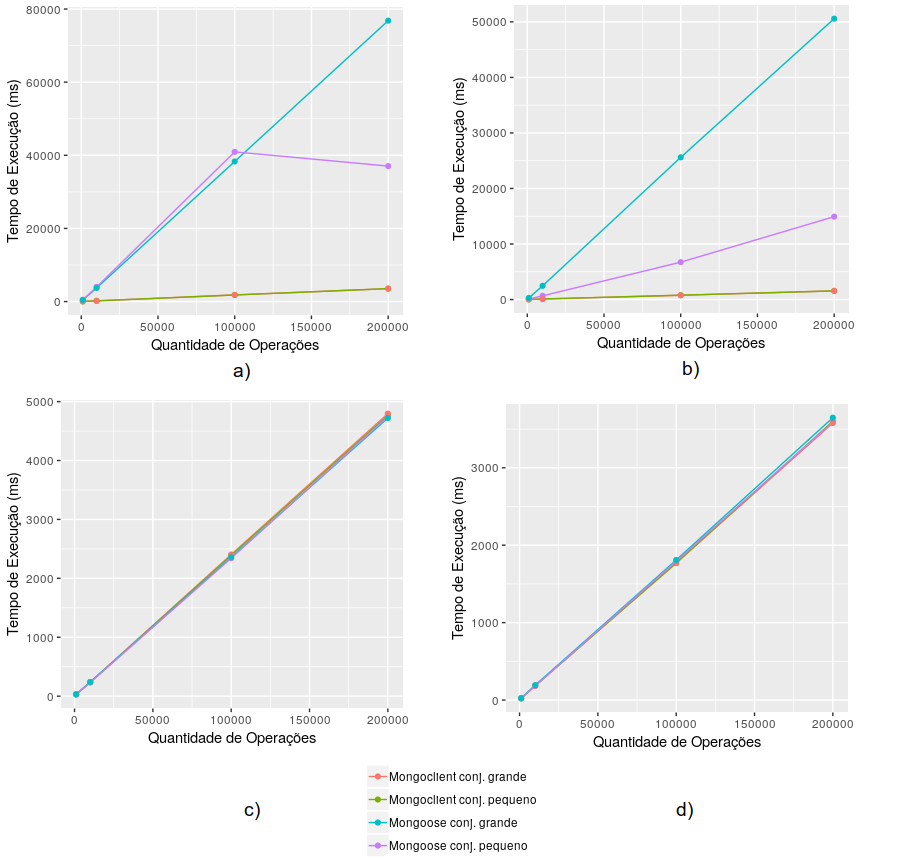
\includegraphics[width=0.85\textwidth]{images/time}
%\caption{Comparison of the use of drivers with the application of CRUD operations in relation to the runtime.}
%\label{fig:time}
%\end{figure}

\begin{figure}[!ht]
    \centering
    \subfloat[] {
        \begin{minipage}[1\width]{0.37\textwidth}
            \centering
            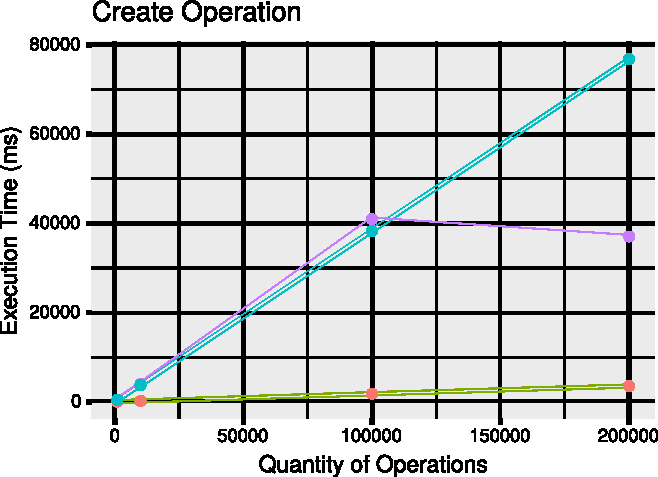
\includegraphics[width=1\textwidth]{images/difftime-create.pdf}
            \label{fig:time-a}
        \end{minipage}
    }
    \subfloat[] {
        \begin{minipage}[1\width]{0.37\textwidth}
            \centering
            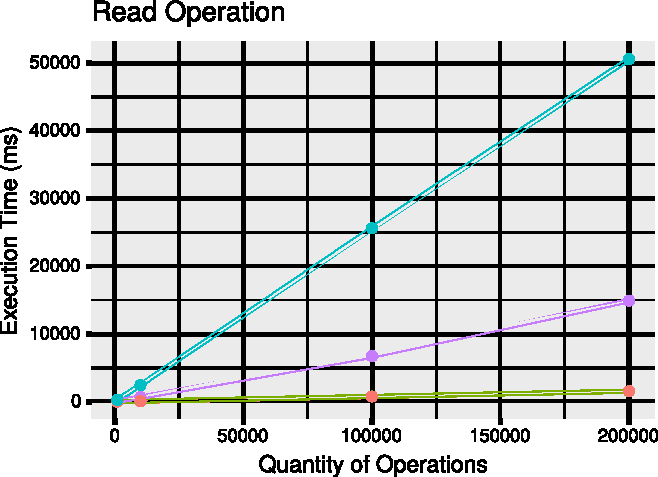
\includegraphics[width=1\textwidth]{images/difftime-read.pdf}
            \label{fig:time-b}
        \end{minipage}}
    \newline
    \subfloat[] {
        \begin{minipage}[1\width]{0.37\textwidth}
            \centering
            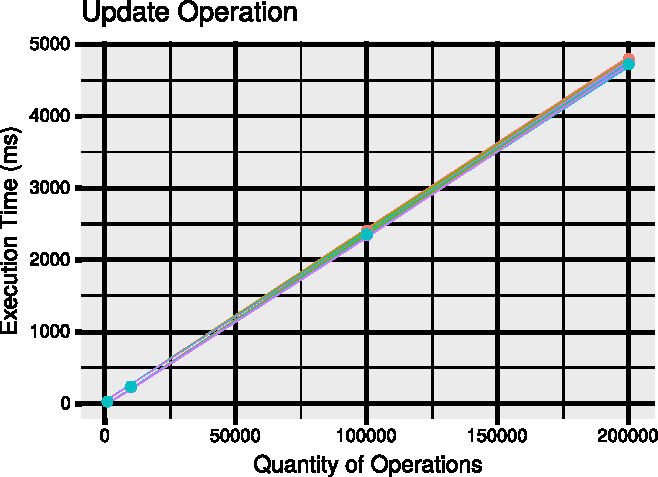
\includegraphics[width=1\textwidth]{images/difftime-update.pdf}
            \label{fig:time-c}
        \end{minipage}}   
    \subfloat[] {
        \begin{minipage}[1\width]{0.37\textwidth}
            \centering
            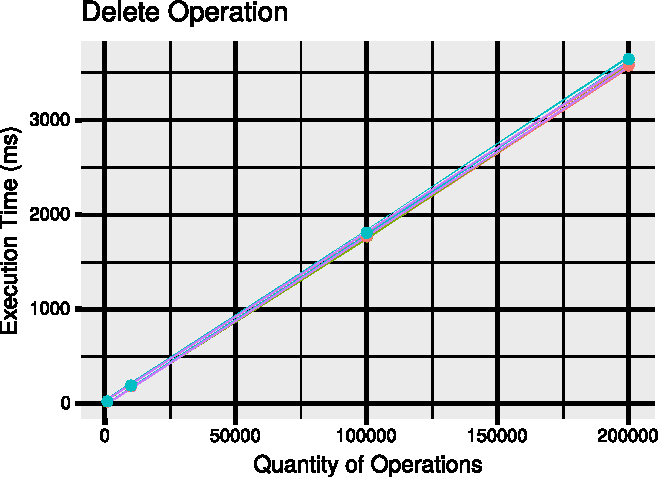
\includegraphics[width=1\textwidth]{images/difftime-delete.pdf}
            \label{fig:time-d}
        \end{minipage}} 
        \newline
    \subfloat {
        \begin{minipage}[1\width]{0.12\textwidth}
            \centering
            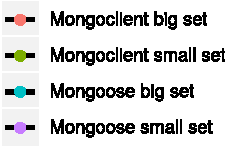
\includegraphics[width=1\textwidth]{images/legend.pdf}
        \end{minipage}} 
    \caption{Comparison of the use of drivers with the application of CRUD operations in relation to the runtime.}
    \label{fig:time}
\end{figure}

Figure~\ref{fig:time} graphically illustrates the execution time when performing CRUD operations contrasting the use of both drivers. Considering the execution time for insert operations - Figure~\ref{fig:time-a}, it was identified that the execution time with the use of driver Mongoose was longer for both sets, compared to the use of MongoClient, which showed no significant differences between the sets. It can also be noted that when manipulating the small dataset using Mongoose, there was a drop in execution time from 100,000 insert operations. A possible factor that justifies this behavior is the occurrence of set splitting in the insert operation when the quantity exceeds 100,000 items, according to MongoDB documentation, however, this does not occur for the large data set.

Considering the execution time for Search operations - Figure~\ref{fig:time-b}, using MongoClient resulted in lower execution time for both sets compared to using Mongoose. Using Mongoose in this case, the executions for both sets exhibit increasing and proportional behavior to the detriment of the record size difference. Finally, from a processing time perspective, when analyzing test results for both update operations - Figure~\ref{fig:time-c} and deletion operations - Figure~\ref{fig:time-d}, similar behaviors were observed with the use of both drivers.

%\begin{figure}[ht]
%    \centering
%    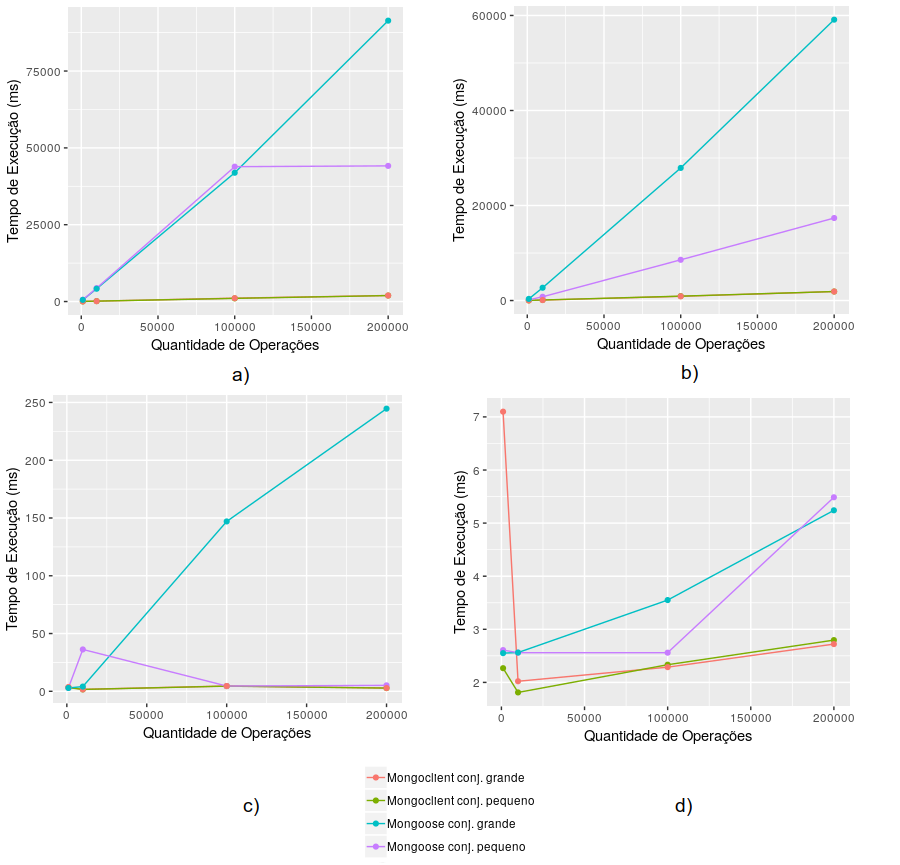
\includegraphics[width=0.85\textwidth]{images/cpuusage}
%    \caption{Comparativo de operações CRUD em relação ao consumo de CPU.}
%	 \caption{Comparison of the use of drivers with the application of CRUD operations in relation to the CPU consumption.}
%    \label{fig:cpuusage}
%\end{figure}

\begin{figure}[!ht]
    \centering
    \subfloat[] {
        \begin{minipage}[1\width]{0.37\textwidth}
            \centering
            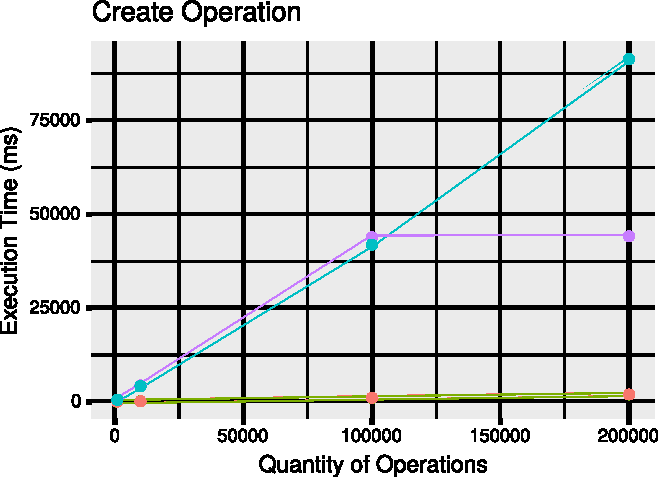
\includegraphics[width=1\textwidth]{images/cpuusage-create.pdf}
            \label{fig:cpu-a}
        \end{minipage}
    }
    \subfloat[] {
        \begin{minipage}[1\width]{0.37\textwidth}
            \centering
            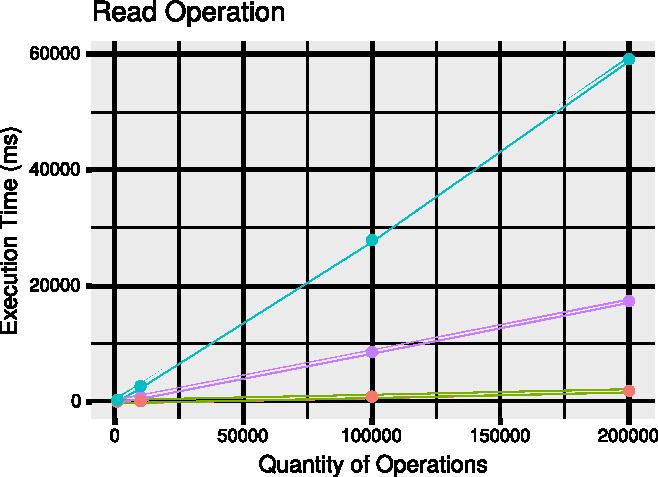
\includegraphics[width=1\textwidth]{images/cpuusage-read.pdf}
            \label{fig:cpu-b}
        \end{minipage}}
    \newline
    \subfloat[] {
        \begin{minipage}[1\width]{0.37\textwidth}
            \centering
            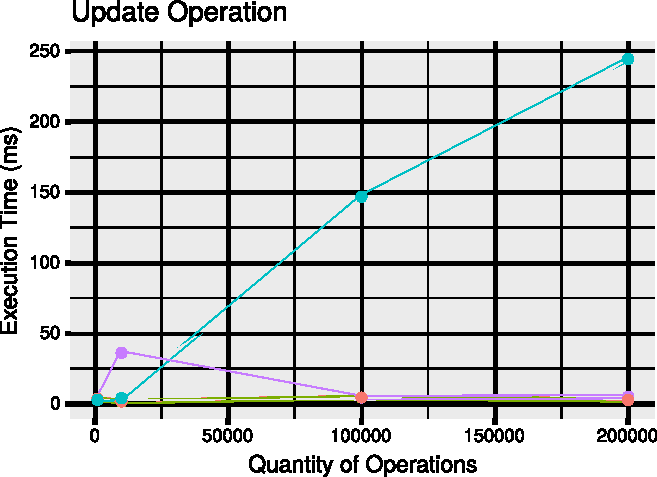
\includegraphics[width=1\textwidth]{images/cpuusage-update.pdf}
            \label{fig:cpu-c}
        \end{minipage}}   
    \subfloat[] {
        \begin{minipage}[1\width]{0.37\textwidth}
            \centering
            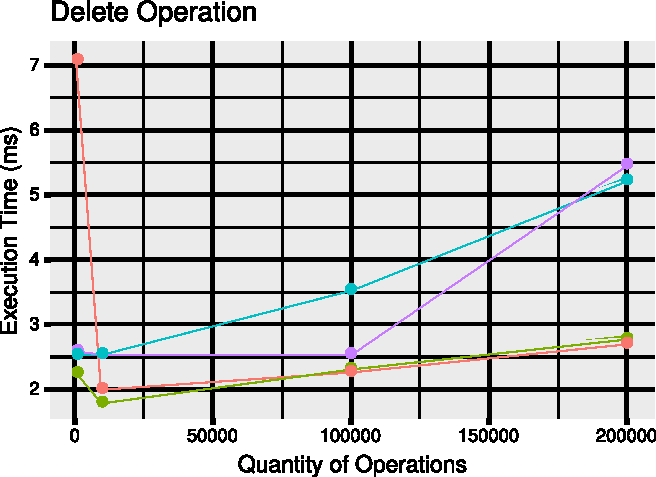
\includegraphics[width=1\textwidth]{images/cpuusage-delete.pdf}
            \label{fig:cpu-d}
        \end{minipage}} 
    \newline
    \subfloat {
        \begin{minipage}[1\width]{0.12\textwidth}
            \centering
            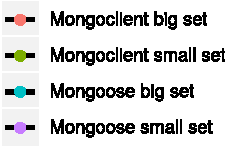
\includegraphics[width=1\textwidth]{images/legend.pdf}
        \end{minipage}} 
    \caption{Comparison of the use of drivers with the application of CRUD operations in relation to the CPU consumption.}
    \label{fig:cpuusage}
\end{figure}

Figure~\ref{fig:cpuusage} graphically illustrates CPU consumption when performing CRUD operations by contrasting the use of both drivers.
Similarly to the previous analysis, for insert operations - Figure~\ref{fig:cpu-a} and fetch - Figure~\ref{fig:cpu-b}, MongoClient usage provides significantly lower average CPU consumption time in both sets, to the detriment of the high consumption time presented by Mongoose. For insertion, it also presents the exception case for 200,000 operations, whose possible justification is similar to the previous analysis.

Figure~\ref{fig:cpu-c} illustrates the CPU consumption when performing update operations, where it can be observed that using the Mongoose driver with a larger record set had a longer CPU consumption time, unlike the others, which were similar and with a shorter time, even with oscillations.
Importantly, the processing time of all runs was less than 250 ms.
In Figure~\ref{fig:cpu-d}, CPU consumption is shown when performing deletion operation, each execution presented relatively unstable behavior, in which the use of driver MongoClient had a higher CPU consumption time, however, there is no significant difference because all executions obtained processing time of less than 10 ms.

%\begin{figure}[!ht]
%    \centering
%    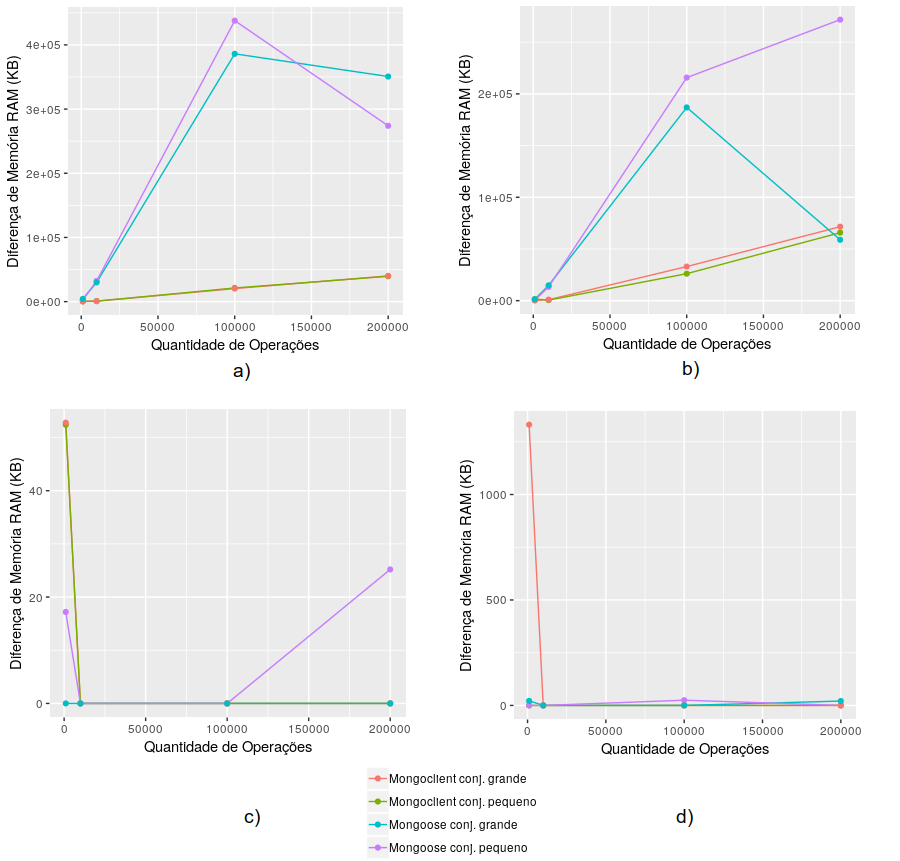
\includegraphics[width=0.85\textwidth]{images/memory}
%    \caption{Comparativo de operações em relação ao uso de memória.}
%	 \caption{Comparison of the use of drivers with the application of CRUD operations in relation to the Memory consumption.}
%    \label{fig:memory}
%\end{figure}

\begin{figure}[!ht]
    \centering
    \subfloat[] {
        \begin{minipage}[1\width]{0.37\textwidth}
            \centering
            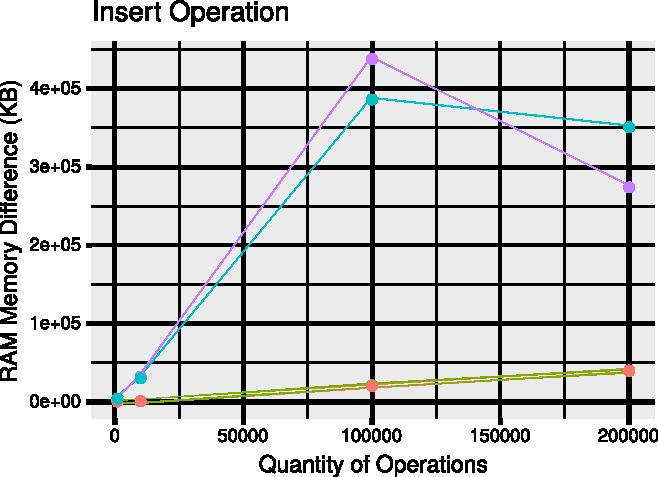
\includegraphics[width=1\textwidth]{images/memory-create.pdf}
            \label{fig:memory-a}
        \end{minipage}
    }
    \subfloat[] {
        \begin{minipage}[1\width]{0.37\textwidth}
            \centering
            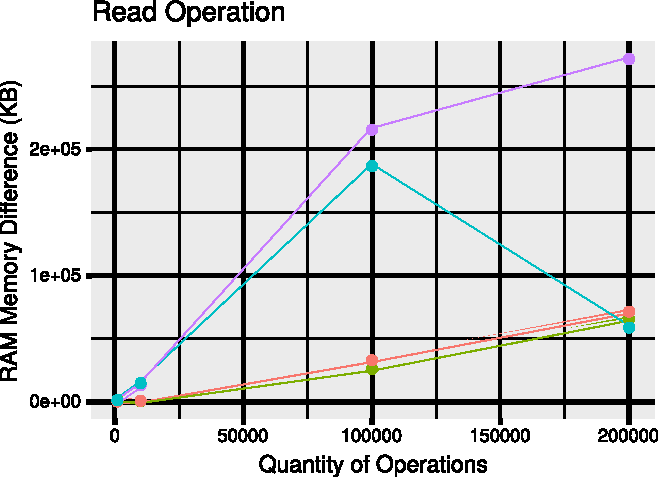
\includegraphics[width=1\textwidth]{images/memory-read.pdf}
            \label{fig:memory-b}
        \end{minipage}}
    \newline
    \subfloat[] {
        \begin{minipage}[1\width]{0.37\textwidth}
            \centering
            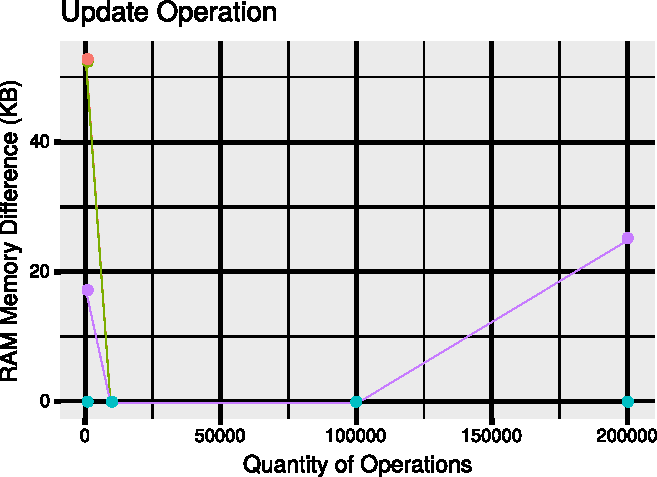
\includegraphics[width=1\textwidth]{images/memory-update.pdf}
            \label{fig:memory-c}
        \end{minipage}}   
    \subfloat[] {
        \begin{minipage}[1\width]{0.37\textwidth}
            \centering
            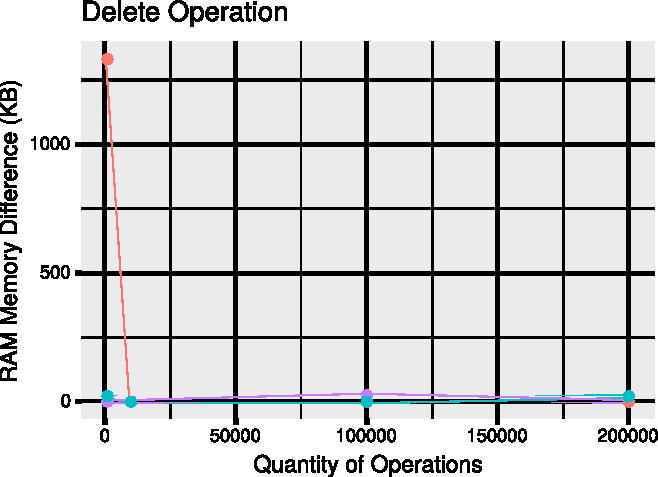
\includegraphics[width=1\textwidth]{images/memory-delete.pdf}
            \label{fig:memory-d}
        \end{minipage}} 
    \newline
    \subfloat {
        \begin{minipage}[1\width]{0.12\textwidth}
            \centering
            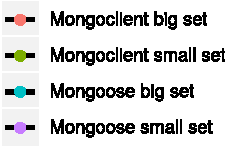
\includegraphics[width=1\textwidth]{images/legend.pdf}
        \end{minipage}} 
    \caption{Comparison of the use of drivers with the application of CRUD operations in relation to the Memory consumption.}
    \label{fig:memory}
\end{figure}

Figure~\ref{fig:memory} graphically illustrates RAM consumption when performing CRUD operations contrasting the use of both drivers.
Figures~\ref{fig:memory-a} and~\ref{fig:memory-b} respectively show the memory consumptions for insert and search operations, in which a pattern of memory usage cannot be identified, however it can be identified that predominantly driver Mongoose has a higher memory consumption in operations performed on both sets to the driver MongoClient cases.
For both operations, there is additional memory usage of around 30 to 40MB.

Finally, Figures~\ref{fig:memory-c} and~\ref{fig:memory-d} respectively show the memory consumption when performing an update and delete operations, do not show standardization for both drivers and sets. 
Despite having some points of instability, it is possible to notice that such operations consume little additional memory, approximately 1MB or less, even considering the oscillation peaks.

\section{Analysis}
\label{section:discussao}

This section presents the analysis of the results obtained, which are described from the perspective of the descriptive research questions in the Section~\ref{section:experimento}.

\subsection{~\emph{RQ1 -- Does the driver selection impact on application performance under time execution?}}
%\subsection{Análise -- QP1}
\label{q1}

Regarding RQ1, in general, the tests performed using the Mongoose driver had a higher execution time compared to using MongoClient in two operations, while in the other operations the performance was similar.
Thus, from the average execution time perspective of each operation performed on the MongoDB database, driver choice can impact performance, with MongoClient being the best choice for a Node.js application that makes use of MongoDB if time execution is a critical factor for this application.

\subsection{~\emph{RQ2 -- Does the driver selection affect application performance under CPU usage?}}
%\subsection{Análise -- QP2}
\label{q2}

As in RQ1, tests performed using MongoClient had lower CPU consumption time compared to Mongoose in both sets, mainly for insert and fetch operations, while in the other operations (update and delete), it was also recorded better performance, but to a lesser extent.
In short, in terms of processing time, driver choice can influence performance, also presenting MongoClient as the best option for a Node.js application that makes use of MongoDB.

\subsection{~\emph{RQ3 -- Does the driver selection impact application performance under RAM memory consumption?}}
%\subsection{Análise -- QP3}
\label{q3}

Considering RQ3, we have that for insert and search operations, in most execution cases, driver Mongoose has higher memory consumption, while for update and delete operations there are no significant differences.
However, it is noteworthy that in none of the comparisons there was stable behavior
Thus, in terms of memory consumption, the choice of driver does not significantly impact all operations, despite the lower consumption by driver MongoClient.

\subsection{Overview}
\label{qgeral}

In general, the data obtained indicate that insertion and search operations are the most costly in execution time, in the worst cases approximately 70,000 to 80,000 ms, while the others are less than 5,000 ms.
From the perspective of CPU consumption time the same analysis is also used, the operations indicate approximate proportionality compared to the total execution time.
As for memory usage, both operations are also costly, even if nonlinear, at levels close to 30 to 40MB, to the detriment of other operations with usage close to or less than 1MB.

Considering the average difference in record size of the adopted dataset, driver MongoClient was indifferent, showing no significant oscillations, while Mongoose presented performance directly proportional to the record size.

In terms of driver comparison, MongoClient performed more stable from the perspective of all adopted metrics than Mongoose. Therefore, it is concluded that, under the exclusive performance criterion, MongoClient presents itself as the best option for the Mongoose. It should be noted that if any additional resources provided by one of the options, such as data verification or ease of implementation, are relevant factors, the choice should be reevaluated, however, this study is quantitative and is not intended to measure the use of additional resources. which may vary from context and application used.

%\section{Ameaças à Validação}
%\label{section:limitacoes}

%Esta seção apresenta as possíveis ameaças que podem comprometer os resultados desse estudo comparativo.
%Como ameaça à validação interna desse estudo tem a etapa da obtenção dos dados quantitativos quanto às análises conduzidas, desse modo, durante a execução dos testes, todos esses foram conduzidos repetidamente e de modo subsequente para que nenhuma interferência pudesse ser adicionada.

%Como ameaça à validação externa, tem-se o conjunto de dados selecionado, o qual está diretamente atrelado aos resultados numéricos obtidos, porém análise é baseado na comparação relativa dos resultados, além a aplicação de teste foi projetada de modo aceitar um conjunto de dados genérico.

%\section{Trabalhos Relacionados} 
%\label{section:relacionados}

%Este trabalho busca analisar o impacto causado no desempenho de uma aplicação Node.js que faz uso do Banco de Dados~\emph{NoSQL} MongoDB, ao utilizar os dois diferentes drivers disponíveis para o Banco de Dados em questão. Nosso trabalho está situado como único presente na literatura com investigação nessa perspectiva, uma vez que os demais trabalhos investigam outros aspectos relacionados ao MongoDB como por exemplo: comparação de desempenho com outros bancos de dados e influência na performance do banco de dados ao utilizar diferentes modelagens de dados. A seguir são descritos alguns desses trabalhos.

%Uma análise quantitativa do desempenho entre o MongoDB e o Banco de Dados Relacional MySQL~\cite{patil:2017}. Como resultados, foi constatado que o MongoDB apresentou melhor performance em operações de inserção e recuperação se comparado com o MySQL. 
%Em um estudo análogo~\cite{jung:2015}, foi demonstrado que o MongoDB possui em geral desempenho superior ao Banco de Dados Relacional PostgreSQL, considerando operações CRUD, entretanto o desempenho do PostgreSQL é superior quando é utilizado um modelo de dados estruturado.

%Em outro estudo, por meio de uma aplicação web é comparado o desempenho da utilização integral do MySQL e de um modelo híbrido de MySQL e MongoDB~\cite{ongo:2018}. 
%Em seus resultados, é expresso que o banco de dados híbrido obteve desempenho mais alto em operações de leitura e gravação se comparado ao MySQL de modo isolado. 
%Além disso, o modelo híbrido consome menos disco, contudo consome mais memória se comparado com a utilização integral do MySQL, o consumo de CPU não apresenta diferença significativa entre as duas abordagens. 
%Um possível trabalho futuro poderia comparar o modelo Híbrido com a utilização integralmente do MongoDB e investigar o desempenho, consumo de Disco, Memória RAM e CPU.

%Além disso, foi verificado a variação do desempenho do Banco de Dados~\emph{NoSQL} MongoDB na perspectiva de dois estilos de modelagem diferentes: incorporação de documentos e normalização em coleções. Os resultados demonstraram que o modelo de dados incorporado do MongoDB oferece um desempenho superior e muito mais consistente em todas as consultas em comparação com o modelo de dados normalizado do MongoDB~\cite{kanade2014study}.

\section{Final Remarks}
\label{section:consideracoes}

This paper presents a study that analyzes the influence of using drivers, contrasting the use of two distinct drivers, MongoClient and Mongoose, on the performance of a Node.js application that makes use of the NoSQL MongoDB database.%Este artigo apresenta um estudo analisando o desempenho de uma aplicação Node.js que faz uso do Banco de Dados \emph{NoSQL} MongoDB contrastando a utilização de dois~\emph{drivers} distintos: \emph{MongoClient} e \emph{Mongoose}.
A performance analysis study was conducted considering aspects such as runtime, CPU time, and RAM usage in performing CRUD operations. Also, the impacts resulting from the variation in the average size of the records in the dataset were compared.

In general, from the quantitative results, it was found that the performance of a Node.js application integrated with MongoDB when using driver MongoClient is generally better compared to using driver Mongoose, especially under the runtime and CPU consumption and, less significantly, RAM consumption, considering an application developed in a Node.js environment.

As an additional contribution, there is the implementation and availability of the testing tool, in order to enable the execution of future analyzes in Node.js environments.

%\begin{table}
%\caption{This is the example table taken out of {\it The
%\TeX{}book,} p.\,246}
%\begin{center}
%\begin{tabular}{r@{\quad}rl}
%\hline
%\multicolumn{1}{l}{\rule{0pt}{12pt}
%                   Year}&\multicolumn{2}{l}{World population}\\[2pt]
%\hline\rule{0pt}{12pt}
%8000 B.C.  &     5,000,000& \\
%  50 A.D.  &   200,000,000& \\
%1650 A.D.  &   500,000,000& \\
%1945 A.D.  & 2,300,000,000& \\
%1980 A.D.  & 4,400,000,000& \\[2pt]
%\hline
%\end{tabular}
%\end{center}
%\end{table}
%
%
% ---- Bibliography ----
%
%\begin{thebibliography}{6}
%

%\bibitem {smit:wat}
%Smith, T.F., Waterman, M.S.: Identification of common molecular subsequences.
%J. Mol. Biol. 147, 195?197 (1981). \url{doi:10.1016/0022-2836(81)90087-5}

%\bibitem {may:ehr:stein}
%May, P., Ehrlich, H.-C., Steinke, T.: ZIB structure prediction pipeline:
%composing a complex biological workflow through web services.
%In: Nagel, W.E., Walter, W.V., Lehner, W. (eds.) Euro-Par 2006.
%LNCS, vol. 4128, pp. 1148?1158. Springer, Heidelberg (2006).
%\url{doi:10.1007/11823285_121}

%\bibitem {fost:kes}
%Foster, I., Kesselman, C.: The Grid: Blueprint for a New Computing Infrastructure.
%Morgan Kaufmann, San Francisco (1999)

%\bibitem {czaj:fitz}
%Czajkowski, K., Fitzgerald, S., Foster, I., Kesselman, C.: Grid information services
%for distributed resource sharing. In: 10th IEEE International Symposium
%on High Performance Distributed Computing, pp. 181?184. IEEE Press, New York (2001).
%\url{doi: 10.1109/HPDC.2001.945188}

%\bibitem {fo:kes:nic:tue}
%Foster, I., Kesselman, C., Nick, J., Tuecke, S.: The physiology of the grid: an open grid services architecture for distributed systems integration. Technical report, Global Grid
%Forum (2002)

%\bibitem {onlyurl}
%National Center for Biotechnology Information. \url{http://www.ncbi.nlm.nih.gov}

%\end{thebibliography}

\bibliographystyle{bibtex/splncs03_unsrt}
\bibliography{sbc-template}

\end{document}
